\section{The Restocking Problem}
\label{sec:problem}

\subsection{Store and robot}
The store is a $4\times4$ grid with a depot at $(0,0)$ and two shelves, each holding up to three units. The robot carries at most two units. At every step it chooses one of seven actions: move up, down, left or right, restock the shelf it stands on, reload at the depot, or wait. Restocking moves as many units as fit from the robot onto the shelf; reloading fills the robot, but only at the depot. After the action, each shelf that still has stock independently loses one unit with probability $p=0.12$, so the two shelves together see on average one sale every four steps. A run is cut after $T=200$ steps. The store does not close at that point, so the cut is a time limit and not a terminal state; Section~\ref{sec:learning} returns to why this distinction matters.

Where the two shelves stand is decided by a layout seed. Ten layouts (seeds 0--9) are used throughout, and each acts as one independent replicate of every experiment. They differ a great deal in difficulty (Fig.~\ref{fig:layouts}): when both shelves are close to the depot almost no sale is ever lost, but when both are five or six cells away the robot cannot keep up with demand.

\begin{figure}[t]
\centering
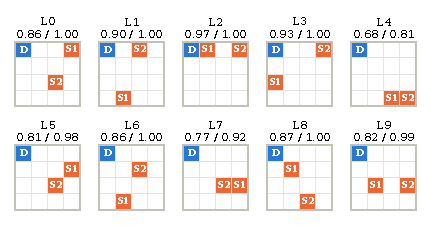
\includegraphics[width=\columnwidth]{layouts}
\caption{The ten store layouts (D: depot; S1, S2: shelves). Each title gives the layout, its optimal service level and the travel-time bound of Section~\ref{sec:bound}.}
\label{fig:layouts}
\end{figure}

\subsection{State}
The Gymnasium observation has eight entries: robot position, units carried, the two stock levels, the number of steps since each shelf was last restocked, and a time-of-day clock. Only the first five affect what happens next. Time since a visit adds nothing once the stock level itself is observed, and demand does not vary with the time of day. The tuple
\begin{equation}
s=(x,\,y,\,c,\,\sigma_1,\,\sigma_2)
\end{equation}
of position, carried units and stock levels is therefore a Markov state, with $4\cdot4\cdot3\cdot4\cdot4=768$ values. Every agent in this study, tabular or neural, observes exactly this tuple. In Review~II the tabular agents also carried a two-valued time-of-day bit, which doubled their table without telling them anything.

\subsection{What the store pays for}
The objective is defined first, before any reward used for training. The store loses sales when a shelf is empty and pays for robot travel, so the objective reward is
\begin{equation}
r_{\text{obj}} = -8\,n_{\text{empty}} - 0.1\,m ,
\label{eq:objective}
\end{equation}
where $n_{\text{empty}}$ counts shelves at zero stock after demand and $m\in\{0,1\}$ records whether the robot moved. A sale is lost only when a customer arrives at an empty shelf, which happens with probability $p$ per step, so the expected number of lost sales is proportional to the number of empty shelf-steps. The weight 0.1 says that 80 moves cost as much as one shelf standing empty for one step; Section~\ref{sec:frontier} examines what that choice implies. Every policy in this paper is scored on~\eqref{eq:objective}, whatever reward it was trained on.

\subsection{The proposal reward}
The project proposal trained agents on a richer signal:
\begin{multline}
r_{\text{prop}} = r_{\text{obj}} - 0.2 - 1\cdot\mathbb{1}[\text{invalid}] + 10\cdot\mathbb{1}[\text{restock}, \sigma>0] \\
+ 5\cdot\mathbb{1}[\text{restock}, \sigma=0] + 2\cdot\mathbb{1}[\text{closer}] ,
\label{eq:proposal}
\end{multline}
with a constant step cost, a penalty for a restock or reload that cannot happen, a bonus for restocking (halved if the shelf was already empty), and a bonus whenever a step reduces the distance to the lowest-stock shelf.

The closer bonus can be gamed. A step toward the target earns $2-0.1-0.2=+1.7$, while a step away costs only $-0.3$, so walking back and forth earns $+1.4$ every two steps where waiting earns $-0.4$. A reward that pays for progress without charging for regress makes loops profitable; Randl{\o}v and Alstr{\o}m observed exactly this when a shaped bicycle controller learned to ride in circles~\cite{randlov1998}. Whether the loop is worth exploiting once stockouts are taken into account is not obvious, and Section~\ref{sec:audit} settles it exactly.

\subsection{Potential-based alternatives}
Ng, Harada and Russell showed that a shaping term of the form
\begin{equation}
F(s,s') = \gamma\,\Phi(s') - \Phi(s)
\label{eq:pbrs}
\end{equation}
leaves the optimal policy unchanged for any bounded potential $\Phi$, because the shaped optimal action values are $Q^\ast(s,a)-\Phi(s)$~\cite{ng1999}. Two potentials are tested. The first keeps the proposal's guidance signal, the same target and the same magnitude, in potential form:
\begin{equation}
\Phi_{d}(s) = -2\, \lVert \text{pos}(s) - \text{shelf}_{\arg\min_i \sigma_i}\rVert_1 .
\end{equation}
The second adds the restock bonus in potential form,
\begin{equation}
\Phi_{ds}(s) = \Phi_d(s) + 5\,(\sigma_1+\sigma_2) ,
\end{equation}
so a two-unit restock pays about $+9.5$ at the moment it happens, close to the proposal's $+10$. The price is that each random sale now also produces a shaping penalty of $-5\gamma$. The four training rewards are referred to as \emph{Proposal}, \emph{Objective}, \emph{PBRS-d} and \emph{PBRS-ds}.

\subsection{Exact model}
Given $(s,a)$, everything except demand is deterministic, and demand has at most $2^2$ outcomes. The model enumerates them into arrays of successor indices, probabilities and reward components, so any of the rewards above is a linear combination of stored arrays. The model was checked against the simulator in three ways, all kept as unit tests: every successor observed in 6{,}000 random transitions exists in the model with the same reward under all four rewards; empirical successor frequencies over 20{,}000 draws agree with the model's probabilities to within four standard errors; and the new simulator, run with the proposal reward, reproduces the Review~II environment to $10^{-15}$ for random action sequences.

\subsection{Exact evaluation and the normalised score}
\label{sec:score}
Because every agent acts on the Markov state, any trained agent, whether a Q-table or a neural network, can be written as a policy $\pi$ over the 768 states. Pushing the start-state distribution forward, $d_{t+1}=d_t P_\pi$, gives the exact expected value of every metric over a 200-step run with no sampling noise. The model is used only to measure; no learner ever sees it. As a cross-check, every final policy is also simulated on 100 demand sequences never used in training; Section~\ref{sec:results} shows that the two measurements agree.

Raw returns from different layouts cannot be averaged, because the layouts differ so much in difficulty. Each policy is therefore placed between a uniform-random policy and the best achievable behaviour:
\begin{equation}
\text{score}(\pi) = \frac{J(\pi) - J(\pi_{\text{rand}})}{J^\ast_T - J(\pi_{\text{rand}})} ,
\label{eq:score}
\end{equation}
where $J$ is the expected 200-step sum of~\eqref{eq:objective} from reset and $J^\ast_T$ is its maximum, obtained by backward induction over the 200 steps. A score of 1 is the best any policy can do in expectation.
